\chapter{Problem Analysis \& Solution}
\label{sec:analysis}

We will start by illustrating the input to our visualization problem.

Our input are two homologous triangle meshes which are to be compared. In order to clearly distinguish between these two meshes, we will call one of them the {\it primary mesh} and the other one will be the {\it reference mesh}. The mesh which carries the visualization is always the {\it primary mesh}. For example, Fig. \ref{fig:morpho_example} shows a {\it primary mesh}. The visualization demonstrates how different this {\it primary mesh} is from its {\it reference mesh}.

For the purposes of our arrow-based visualization technique, it is suitable to use difference metrics which can be represented by 3D vectors because these can be directly rendered as arrows. We will restrict ourselves to corresponding vertex distance because this metric used in Morphome3cs suffers from information loss when visualized using only colors. In addition to that, we will also include corresponding vertex distance projected into surface normal despite the fact that this metric only has one dimension. We will use it to compare arrow-based and color-based visualizations. Other metrics can be easily added if needed.

After a difference metric is computed, it is placed as a 3D vector in the corresponding vertex of the {\it primary mesh}. For a better understanding, here is the meaning of such a representation in case of both chosen metrics:

\begin{itemize}
\item For corresponding vertex distance, a vector is placed in the vertex of the {\it primary mesh} and if both meshes were overlaid, its apex would lie in the corresponding vertex of the {\it reference mesh}. This is therefore the most straightforward difference metric and it carries information in multiple dimensions, namely tangential difference and normal difference.
\item For corresponding vertex distance projected into surface normal, the situation is largely similar, only the metric has lost the dimension of tangential difference and is only represented by a single number. When a unit surface normal is multiplied by this number it yields our vector placed in a vertex of the {\it primary mesh}.
\end{itemize}

We will split the vectors into two groups. Vectors which have an acute angle with the positive surface normal will be said to point {\it outwards} and all other vectors will be said to point {\it inwards} (see Fig. \ref{fig:input}). This differentiation will become more meaningful when the meshes in question are for example human faces or other enclosed objects which are very common in geometric morphometrics.

\begin{figure}[h]
\centering
\def\svgwidth{\textwidth}
\input{./illustrations/input_illustration.pdf_tex}
\caption[Input Illustration]{A simplified schema of difference metric vectors. Yellow and blue arrows represent corresponding vertex distance, whereas red arrows show how the distance is projected into surface normal. Yellow arrows point {\it outwards} and blue arrows point {\it inwards}. Notice that all arrows are placed in the {\it primary mesh} and point towards the {\it reference mesh}.}
\label{fig:input}
\end{figure}

To summarize, we are now working with a {\it primary mesh} containing vectors in all its vertices and we are looking for a way to visualize these vectors using an arrow-based visualization. See Fig. \ref{fig:input} for a schema of this situation.

%%-----------------------------------------------------------------------------------------
%% SECTION
%%-----------------------------------------------------------------------------------------
\section{Seeing Mesh Difference as a Vector Field}

If all vectors were drawn directly onto the {\it primary mesh}, the visualization would become too cluttered (see Fig. \ref{fig:meshdiff_unclustered}). We also need a way to group similar vectors together to provide a more global difference visualization which existing color-based visualizations described in the introduction are incapable of.

\begin{figure}[h]
\centering
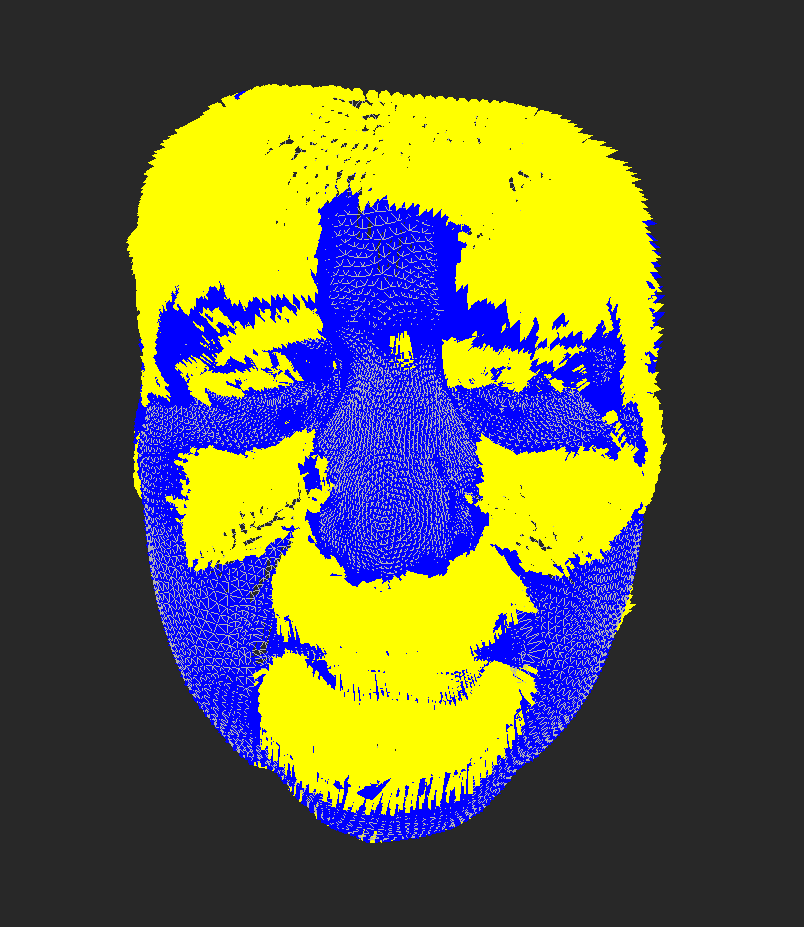
\includegraphics[width=0.5\textwidth]{./img/meshdiff-unclustered_arrows-single.png}
\caption[MeshDiff - Vertex distance visualized by unclustered arrows]{MeshDiff - Vertex distance visualized by unclustered arrows}
\label{fig:meshdiff_unclustered}
\end{figure}

One way to solve this problem is to devise a simple abstraction and use tools available for this abstraction.

Vectors saved in the vertices of a triangle mesh form a discrete bounded vector field. Visualization of discrete vector fields is a very active research area with applications in engineering, molecular modelling and computational fluid dynamics. There exist many scientific papers studying this topic, such as \citet{Telea99}, \citet{Garcke00}, \citet{Du04} or \citet{Peng12}.

Drawing inspiration from these papers we will employ a clustering technique to reduce the number of vectors and subsequently visualize this reduced information.

To summarize again, we are now visualizing a discrete bounded vector field.

%%-----------------------------------------------------------------------------------------
%% SECTION
%%-----------------------------------------------------------------------------------------
\section{Vector Field Clustering}

Clustering in general is a very subjective task (see Fig. \ref{fig:clustering_subjectivity}) and there are numerous approaches to clustering available. For this reason we present an overview of clustering techniques used in vector field visualization to gain a better understanding of which technique might best suit our purposes and why.

\begin{figure}[h]
\centering
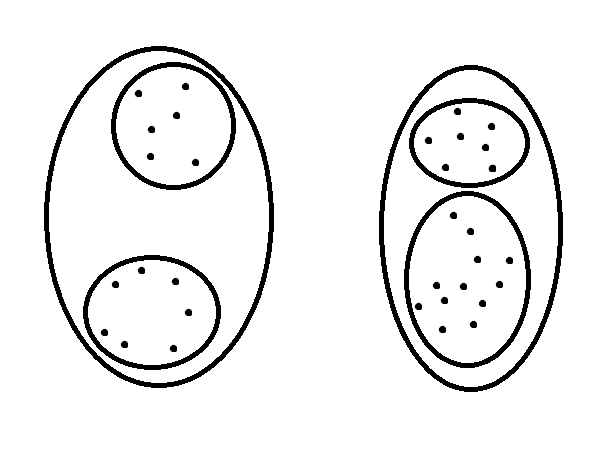
\includegraphics[width=0.6\textwidth]{./img/clustering_subjectivity.png}
\caption[The subjectivity of clustering]{The subjectivity of clustering - are there two or four clusters in the image?}
\label{fig:clustering_subjectivity}
\end{figure}

%%-----------------------------------------------------------------------------------------
\subsection{Overview of Vector Field Clustering Methods}

\citet{Telea99} use hierarchical clustering\footnotemark where neighboring clusters with the lowest clustering error are merged first. Each cluster has a representative vector and during the merge, the weighted average of the two vectors is computed and assigned to the newly formed cluster. In order to compute the clustering error, the paper introduced elliptic iso-error contours\footnotemark. This clustering method is primarily aimed at 2D rectilinear vector fields but can be also used in 3D when the error function is modified appropriately. It is possible to use up to seven parameters to configure the clustering.

\addtocounter{footnote}{-2}
\stepcounter{footnote}\footnotetext{Hierarchical clustering, also called bottom-up clustering, starts with each data point representing an elementary cluster. In each step of the algorithm, two clustering candidates are found from the available clusters according to certain criteria and subsequently merged. Hierarchical clustering creates a binary tree, also called a dendrogram, where each node represents a cluster and has two children from which it was created. Arbitrary number of clusters covering the whole data set can then be obtained by taking roots of disjoint subtrees which, when combined, contain all the leaves of the dendrogram. See Fig. \ref{fig:telea-hierarchical_clustering}.}
\stepcounter{footnote}\footnotetext{Clustering error in \citet{Telea99} is computed by measuring the "distance" between the representative vectors \(v, w\) of the two clusters. The elliptic iso-error contour is an ellipse which has a center on the line determined by \(v\) and intersects the apex of \(w\). All vectors \(w'\) which share the same ellipse have the same "distance" from \(v\). The shape of the ellipse and the location of its center can be controlled by parameters. See Fig. \ref{fig:telea-hierarchical_clustering}.}

\begin{figure}[h]
\centering
	\begin{subfigure}{0.5\textwidth}
	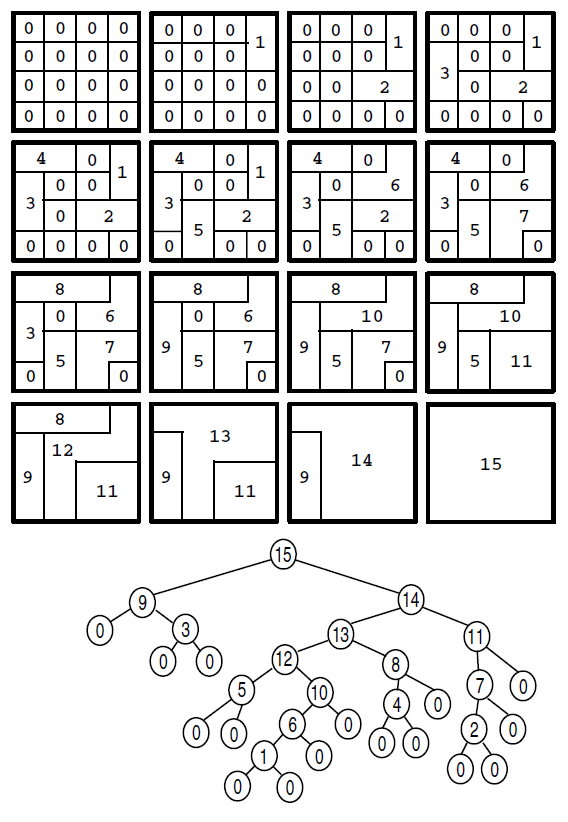
\includegraphics[width=\textwidth]{./img/telea-hierarchical_clustering.PNG}
    \caption{Various clusterings of a data set and the corresponding dendrogram}
	\end{subfigure}
    \qquad
    \begin{subfigure}{0.3\textwidth}
	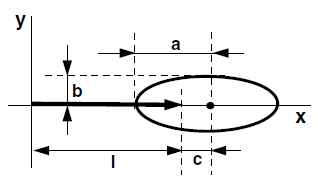
\includegraphics[width=\textwidth]{./img/telea-ellipse-params.PNG}
    \caption{The ellipse and its parameters.}
    
    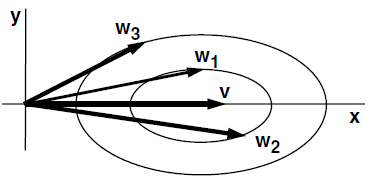
\includegraphics[width=\textwidth]{./img/telea-ellipse-vectors.PNG}
    \caption{The iso-error contours of multiple vectors}
	\end{subfigure}
\caption[The illustration of clustering in \citet{Telea99}]{The illustration of clustering in \citet{Telea99}}
\label{fig:telea-hierarchical_clustering}
\end{figure}

\citet{Garcke00} use a continuous clustering method\footnotemark based on the physical model of \citet{CahnHilliard58} which is used to describe phase separation and coarsening in binary alloys. This model is applied to vector field data which results in a diffusion problem rather than a splitting and merging problem. Their algorithm also assumes an either 2D or 3D rectilinear grid.

\footnotetext{In continuous clustering methods, there is no notion of merging or splitting in each step of the algorithm. Instead, ``a continuous scale of successively coarser cluster sets" is created.}

\citet{Du04} use iterative clustering\footnotemark where Voronoi regions\footnotemark are created around the initial cluster centers and a distance function is applied to each of them. The set of clusters which has the lowest value of the distance function is selected as the final cluster set. This method works with 2D and 3D rectilinear vector fields and can be influenced by two parameters and by the distribution of the initial clusters.

\addtocounter{footnote}{-2}
\stepcounter{footnote}\footnotetext{Iterative clustering algorithms start by assigning the data points to a given number of clusters in a random way or by using a clustering approximation. In each step, the clustering error of all clusters is computed and data points are reassigned in a way which decreases the overall clustering error.}
\stepcounter{footnote}\footnotetext{Voronoi diagram is a partitioning of a plane into regions. The partitioning is done by selecting some initial points as seeds. Then a region is formed around each seed in such a way that a point \(p\) of the plane belongs to the region of seed \(s\) if and only if \(d(p, s') \geq d(p, s) \forall s' \text{ seeds, such that } s' \neq s\).}

\citet{Peng12} use hierarchical clustering similar to \citet{Telea99} with the difference that the clustering is computed on a GPU by encoding a given static view of the vector field into a rasterized image. The computation is then done for this specific image. In order to obtain the clustering error of clusters \(C_1, C_2\), a very simple formula is used:

\begin{equation} \label{eq:clustering_error}
\bm{e}(C_1,C_2) = k_d \cdot \frac{d_{C_1C_2}}{d_{max}} + k_v \cdot \frac{v_{C_1C_2}}{v_{max}} + k_\alpha \cdot \frac{\alpha_{C_1C_2}}{\alpha_{max}} + k_m \cdot \frac{m_{C_1C_2}}{m_{max}}
\end{equation}

where \(k_d + k_v + k_\alpha + k_m = 1\) are weight coefficients. The other components are the following:

\begin{itemize}
\item \(d_{C_1C_2}\) is the Euclidean distance between the positions of the representative vectors of the clusters. The maximum distance \(d_{max}\) is the length of a diagonal of the geometry's bounding box
\item \(v_{C_1C_2}\) is the difference between the lengths of the representative vectors and \(v_{max}\) is the largest length in the whole data set.
\item \(\alpha_{C_1C_2}\) is angle between the representative vectors. The maximum angle is \(\alpha_{max} = 180^\circ\)
\item \(m_{C_1C_2}\) is the sum of the mesh resolutions of the two clusters. \(m_{max}\) is the largest value of \(m\) in the whole data set.
\end{itemize}

The mesh resolution component also differentiates this approach from all others because it represents an approximation of the density of the underlying mesh in a given local area. Including it in the error formula assigns higher error to dense clusters which results in a larger amount of clusters (higher precision) in dense areas of the mesh and a smaller amount of clusters (lower precision) in sparse areas of the mesh. This method is therefore aimed at non-rectilinear 3D vector fields. It has five parameters for user configuration (four weights and the number of clusters to be retrieved from the dendrogram).
%%-----------------------------------------------------------------------------------------
\subsection{Selection Criteria for Our Clustering Method}

For our visualization purposes, we will utilize fragments of the presented clustering methods and introduce certain modifications to accommodate our needs. Here are the criteria for choosing our clustering method:

\begin{itemize}
\item Suitability for the specifics of our vector field
\item Simplicity
\item Ease of user configuration
\end{itemize}

Methods which are suitable for our specific vector field (i.e. a triangle mesh with a vector in each vertex) will help us tailor the clustering process and achieve better results. 

Simple methods will allow us to quickly obtain a baseline which will help us to decide which modifications will improve the algorithm in our conditions. 

Lastly, the ease of user configuration will make our algorithm user-friendly and therefore it will increase the adoption rate.

%%-----------------------------------------------------------------------------------------
\subsection{Our Clustering Method}

We will now describe our clustering method.

\subsubsection{Clustering Algorithm}
\label{sec:analysis_clustering_algorithm}

The preference of hierarchical clustering over other mentioned clustering methods is justified by its simplicity and also the fact that a dendrogram is created during this clustering. This will allow us to quickly react to user requests for various cluster counts with given clustering parameters. Hierarchical clustering will thus make our approach user-friendly. We will, however, introduce one optional condition as to which clusters can be merged together. Our clustering candidates will not only have to be neighbors (as in \citet{Telea99}) but their representative vectors will both have to point either {\it inwards} or {\it outwards} because this distinction may be of importance to the user. On the other hand, we leave this condition as optional because the resulting dendrogram is not a tree but a forest instead. This may result in undesirable artifacts in the visualization because for certain cluster counts, the clustering will not cover the whole data set. See Fig. \ref{fig:forest_dendrogram} for an illustration.

\begin{figure}[h]
\centering
\def\svgwidth{\textwidth}
\input{./illustrations/forest_dendrogram.pdf_tex}
\caption[Forest Dendrogram]{An illustration of clustering with the optional condition enabled and the resulting dendrogram.}
\label{fig:forest_dendrogram}
\end{figure}

We are not going to use the GPU-based approach to clustering computation from \citet{Peng12} because it does not allow the user to view the final visualization from varying angles in real time. In order to support interactive visualization viewing, we will store our vector field in memory and compute the clustering on the whole field in one process instead (as in \citet{Telea99}).

\subsubsection{Clustering Error Function}

We will use the error function presented in \citet{Peng12} (see Eq. \ref{eq:clustering_error}) because it is the only one which assumes vector fields on other than rectilinear grids. Its mesh resolution component makes it suitable to use in the clustering of vector fields on triangle meshes. The function is also simpler and more easily scalable than the elliptic iso-error contours presented in \citet{Telea99} which lead to cube root equations in 3D.

\subsubsection{Cluster Merging}

Besides clustering error computation, merging is the second crucial part of a hierarchical clustering algorithm. In the clustering of vector fields, a representative vector is usually assigned to a newly formed cluster. In our case, this shall be a weighted average of the representative vectors of the child clusters where the weight will be the geometrical area of the given cluster. Geometrical area is a better metric for cluster size than data point count because our underlying triangle mesh is expected to be of varying density.

\subsubsection{Summary}

Our clustering method will use the hierarchical algorithm and CPU-based clustering computation from \citet{Telea99} with the added optional condition of merging only clusters whose representative vectors both point in the same direction - either {\it inwards} or {\it outwards}. We will use the error function from \citet{Peng12} (see Eq. \ref{eq:clustering_error}). Merging of two clusters will be done by computing the area-weighted average of their representative vectors and assigning the resulting vector to the newly formed cluster.

After the clustering step, we are visualizing a set of clusters, each of which has a representative vector which encodes a difference metric averaged across the whole cluster.
%%-----------------------------------------------------------------------------------------
%% SECTION
%%-----------------------------------------------------------------------------------------
\section{Proposed Visualizations}
\label{sec:analysis_visualizations}

Here we present the descriptions of new visualizations. One of them is arrow-based as was our goal and the rest are complementary visualizations leveraging the clustering process in order to enhance the visual appearance and clarity of existing visualization techniques.

%%-----------------------------------------------------------------------------------------
\subsection{Arrows}
\label{sec:arrow_vis}

Once a clustering of a vector field is obtained, representative vectors of all clusters are visualized using 3D arrows. For this purpose we have prepared a simple 3D model of an arrow (see Fig. \ref{fig:arrow_model}) which is copied to the scene at a specific position, angle and scale given by the representative vector and the cluster it belongs to.

\begin{figure}[h]
\centering
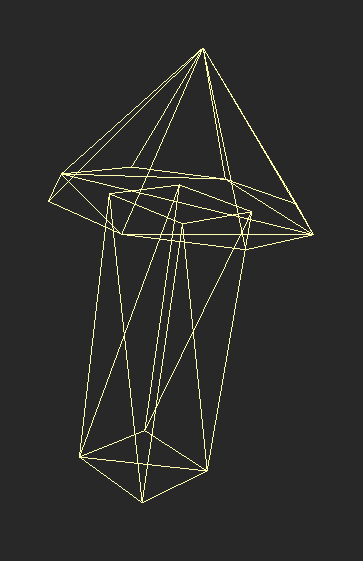
\includegraphics[width=0.3\textwidth]{./img/8sided_arrow.PNG}
\caption[Arrow Model]{Wireframe view of the 3D arrow model}
\label{fig:arrow_model}
\end{figure}

The length of the representative vector influences the length of the 3D arrow. Because the values of the metric can be very close to zero and because their value range is not generally very large, we have decided to set a certain minimum scale and maximum scale, which are adjustable by the user, and map the metric values (vector lengths) to the interval between them. In general, such an approach gives a more visually pleasing and clearer results, especially when the interval is chosen to be large enough.

The scale of the 3D arrows also reflects the geometrical area of the clusters. The larger the clusters are, the thicker the arrows. Areas are again mapped to a user-defined interval for a clearer result. Large clusters are usually important because they represent a general trend in a given area and users should be able to see them more easily and also distinguish them from less important clusters.

Lastly, and most importantly, the direction of the representative vector is reflected directly in the direction of the 3D arrow. In addition to that, Arrows pointing {\it inwards} can have a different color than arrows pointing {\it outwards} to make their differentiation easier for the user.

We have therefore managed to encode three-dimensional information into our visualization.

\begin{figure}[h]
\centering
	\begin{subfigure}{0.3\textwidth}
	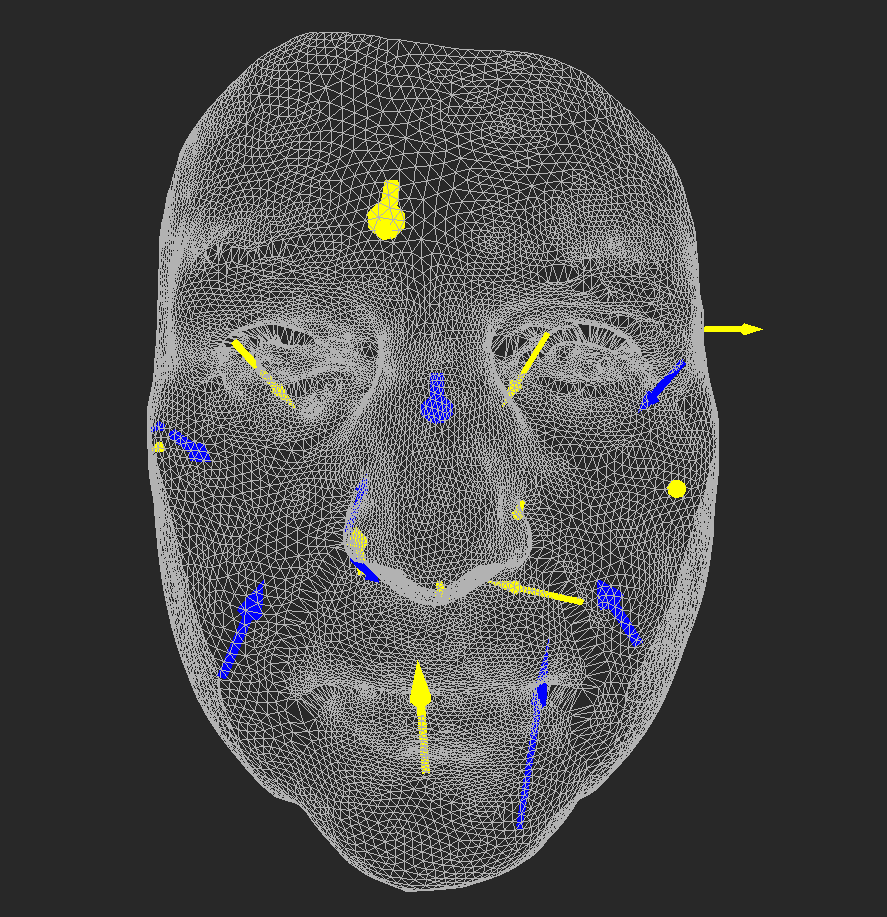
\includegraphics[width=\textwidth]{./img/meshdiff-arrows-interval0_5-5-count20-single.png}
    \caption{Smallest height \& width scale: \(0.5\); largest height \& width scale: 5; cluster count: 20}
    \label{fig:meshdiff_arrows_5-20}
	\end{subfigure}
    \qquad
    \begin{subfigure}{0.3\textwidth}
	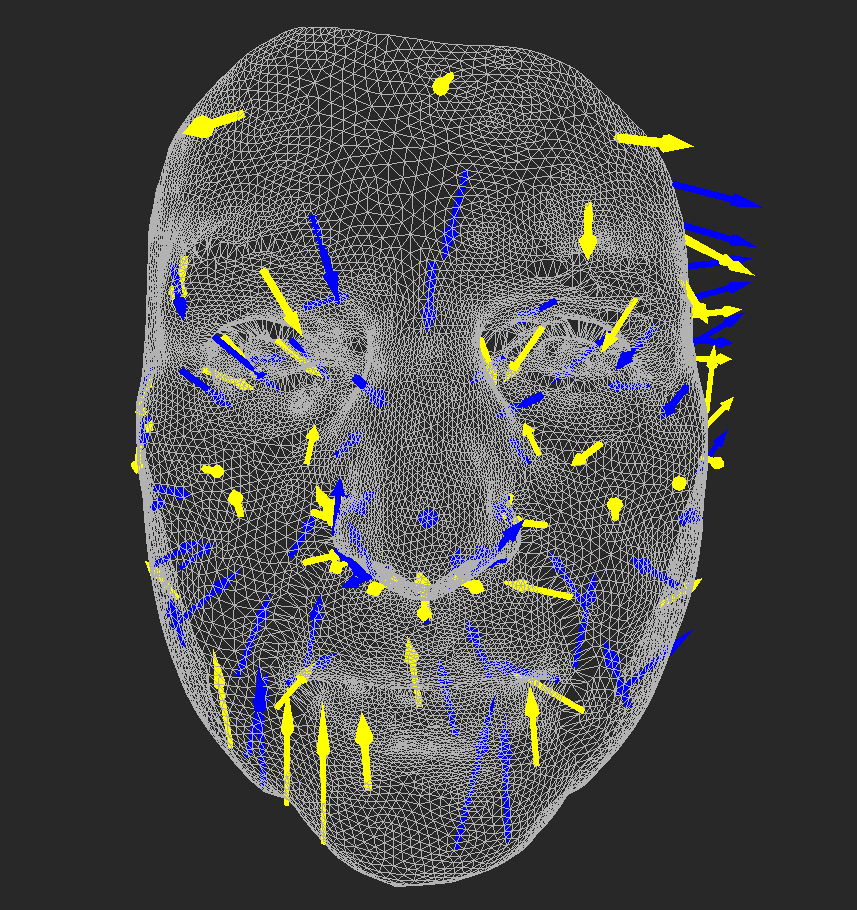
\includegraphics[width=\textwidth]{./img/meshdiff-arrows-interval0_5-5-count125-single.png}
    \caption{Smallest height \& width scale: \(0.5\); largest height \& width scale: 5; cluster count: 125}
    \label{fig:meshdiff_arrows_5-125}
	\end{subfigure}
    
    \begin{subfigure}{0.3\textwidth}
	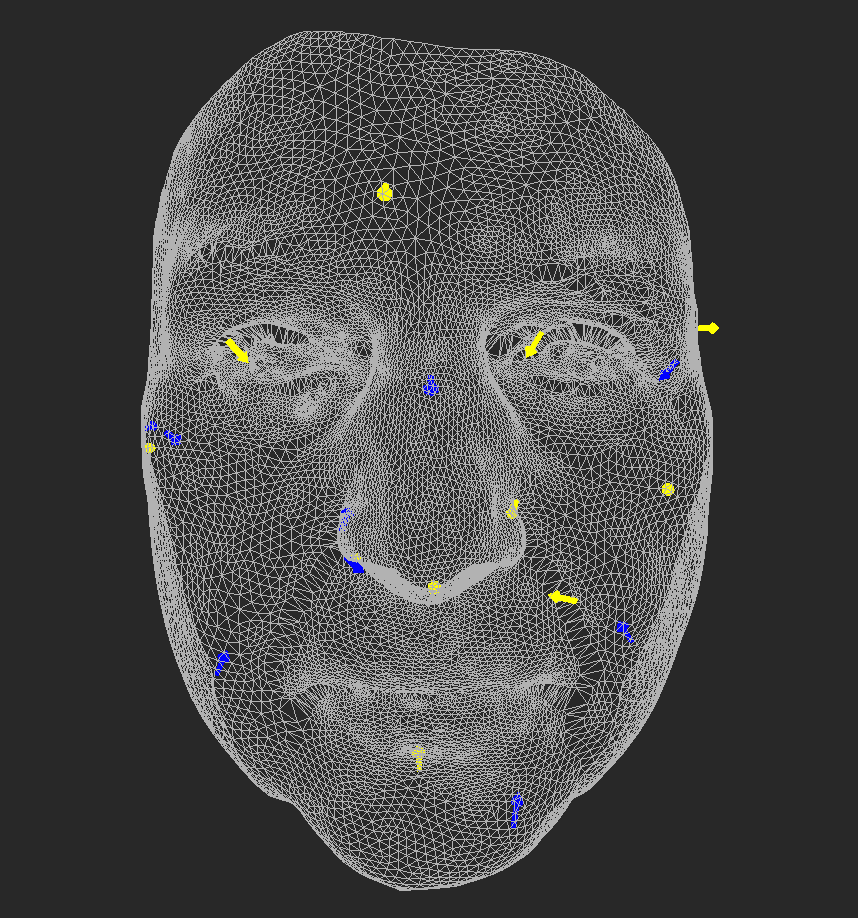
\includegraphics[width=\textwidth]{./img/meshdiff-arrows-interval0_5-1-count20-single.png}
    \caption{Smallest height \& width scale: \(0.5\); largest height \& width scale: 1; cluster count: 20}
    \label{fig:meshdiff_arrows_1-20}
	\end{subfigure}
    \qquad
    \begin{subfigure}{0.3\textwidth}
	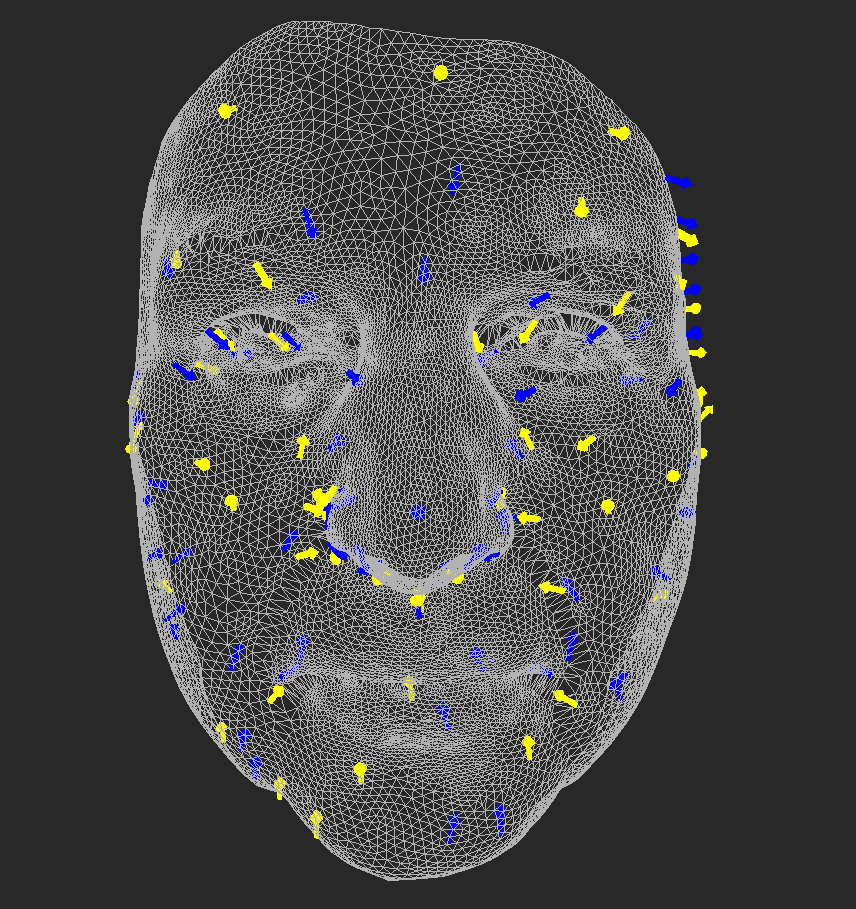
\includegraphics[width=\textwidth]{./img/meshdiff-arrows-interval0_5-1-count125-single.png}
    \caption{Smallest height \& width scale: \(0.5\); largest height \& width scale: 1; cluster count: 125}
    \label{fig:meshdiff_arrows_1-125}
	\end{subfigure}
\caption[MeshDiff - Arrow visualizations with various parameter settings]{MeshDiff - Arrow visualizations with various parameter settings}
\end{figure}

\subsubsection{Expected Performance}

Arrow visualizations combined with clustering are expected to perform well in answering questions about general trends in large parts of the mesh. They are also expected to perform considerably better than color-based visualizations when asking about the direction of the difference, which is particularly important in cases when the difference has a very small angle with the surface of the mesh.
%%-----------------------------------------------------------------------------------------
\subsection{Cluster Color}
\label{sec:analysis-color}

Next, we introduce two color visualizations of clusters: random and metric-based.

Both of these visualizations need to be aware of which mesh vertices belong to a given cluster. Then either a random color is assigned to all vertices in a given cluster or a color based on the length of the representative vector of the cluster is assigned. The former case is basically the original color visualization of a metric, only applied to clusters.

We propose two modes of assigning the color to the vertices based on metrics, the relative mode and the absolute mode. In both modes, a distinct user-defined color hue is assigned to clusters whose representative vectors point {\it inwards} and {\it outwards}. Also, the metric value here is the length of the associated vector. What differentiates the two modes is the shade assigned to clusters of specific metric value.

In the relative mode, the highest and lowest metric values are evaluated first. The lowest value receives black color and the highest value receives the brightest user-defined color. All other values are mapped to this interval and receive a color which is a proportional mixture of the user-defined color and black.

In the absolute mode, black color is assigned to cluster of zero metric value and the brightest color is assigned to clusters of metric value higher or equal than a user-defined value. This allows the user to compare across several visualizations and determine the absolute value of the difference metric more easily.

\begin{figure}[h]
\centering
	\begin{subfigure}{0.3\textwidth}
	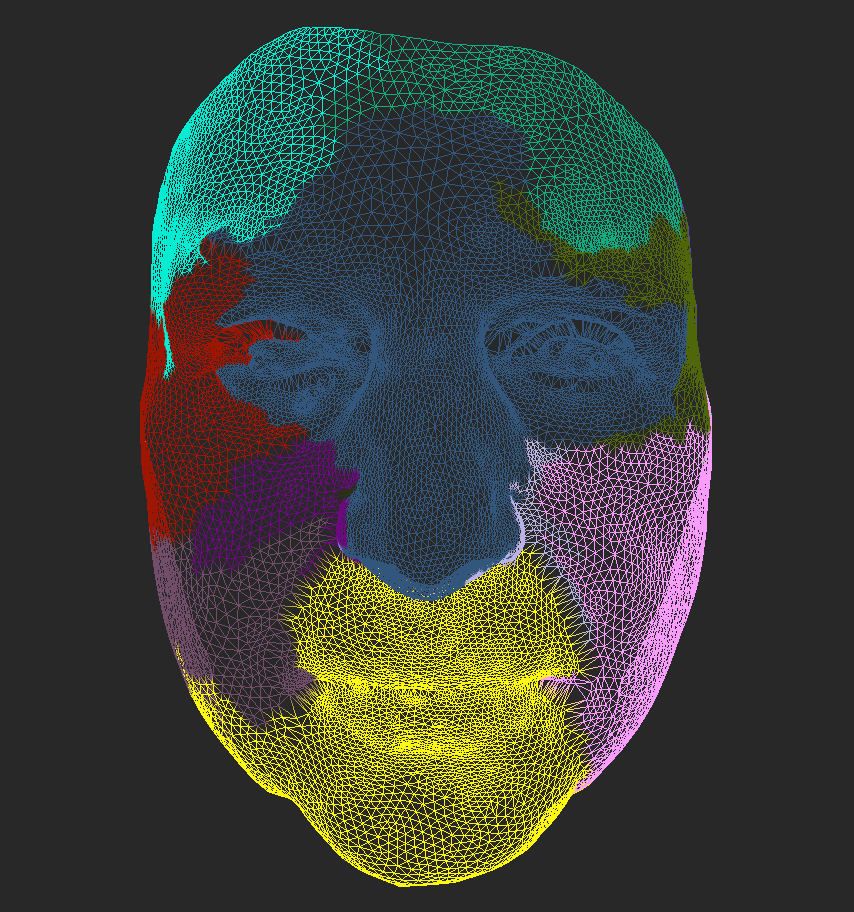
\includegraphics[width=\textwidth]{./img/meshdiff-clustercolor-random.PNG}
    \caption{Random cluster colors}
    \label{fig:meshdiff_clustercolor_random}
	\end{subfigure}
    \qquad
    \begin{subfigure}{0.3\textwidth}
	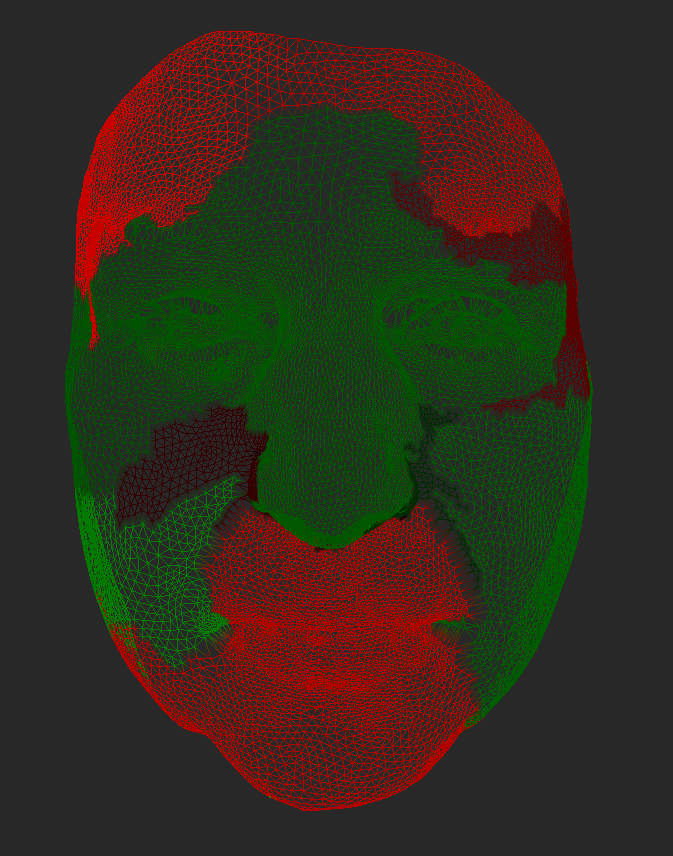
\includegraphics[width=\textwidth]{./img/meshdiff-clustercolor-metric.PNG}
    \caption{Metric-based cluster colors}
    \label{fig:meshdiff_clustercolor_metric}
	\end{subfigure}
    
\caption[MeshDiff - Cluster color visualizations]{MeshDiff - Cluster color visualizations}
\end{figure}

\subsubsection{Expected Performance}

Random cluster color is expected to be used for the purpose of configuring the clustering parameters as the size and the location of the clusters is clearly visible in this case.

Metric-based cluster color is expected to perform well in cases when we have found the most important differences using a more sophisticated visualization and want to present those using a visualization which is as clear as possible.
%%-----------------------------------------------------------------------------------------
\subsection{Thresholding}

For all types of metric-based visualizations including the original color-based ones we present thresholding. The thresholding is either applied to metric values which are too low or clusters whose area is too small. It acts as a high-pass filter and all visualization elements related to the metric or cluster which has not passed the thresholding is excluded from the result.

\begin{figure}[h]
\centering
	\begin{subfigure}{0.3\textwidth}
	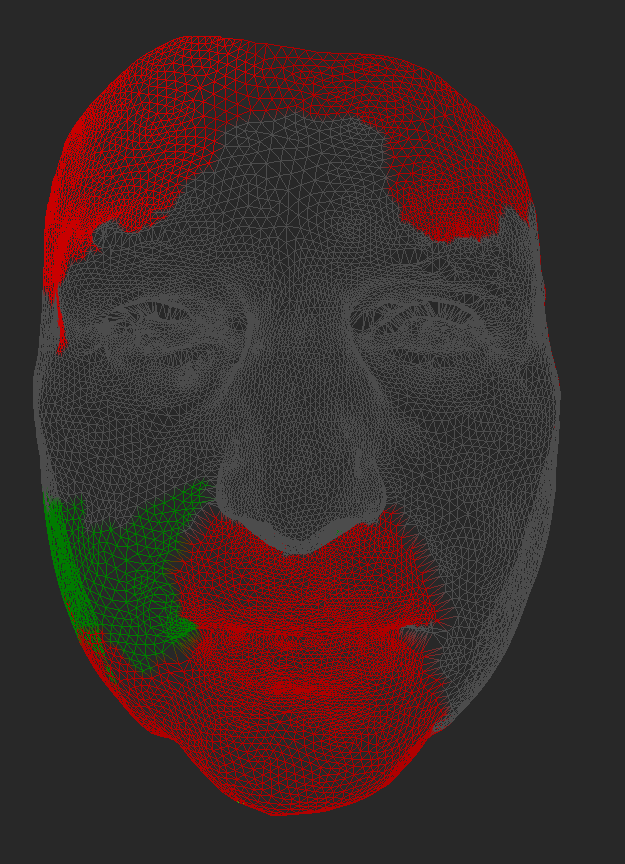
\includegraphics[width=\textwidth]{./img/meshdiff-thresholding-clustercolor-length3.PNG}
    \caption{Clusters with distance less than 3 grayed out}
    \label{fig:meshdiff_thresholding_clustercolor}
	\end{subfigure}
    \qquad
    \begin{subfigure}{0.3\textwidth}
	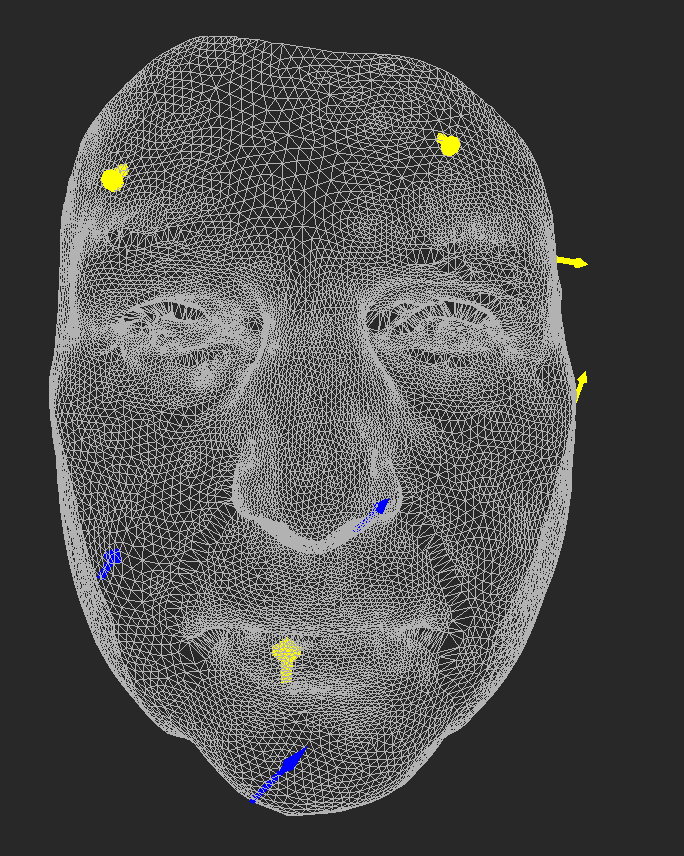
\includegraphics[width=\textwidth]{./img/meshdiff-thresholding-arrows-length3.PNG}
    \caption{Arrows for cluster with distance less than 3 excluded}
    \label{fig:meshdiff_thresholding_arrows}
	\end{subfigure}
    
\caption[MeshDiff - Thresholded visualizations]{MeshDiff - Thresholded visualizations}
\end{figure}

\subsubsection{Expected Performance}

Thresholding is expected to enhance the effect of metric-based cluster color visualizations by performing very well when segmenting and emphasizing a previously discovered difference which is important to the user. It is also expected to help answer questions about the largest differences between two meshes.
%%-----------------------------------------------------------------------------------------
\subsection{Combined Visualizations}

The last visualization type presented in this thesis is the combination of color and arrow visualizations.

\begin{figure}[h]
\centering
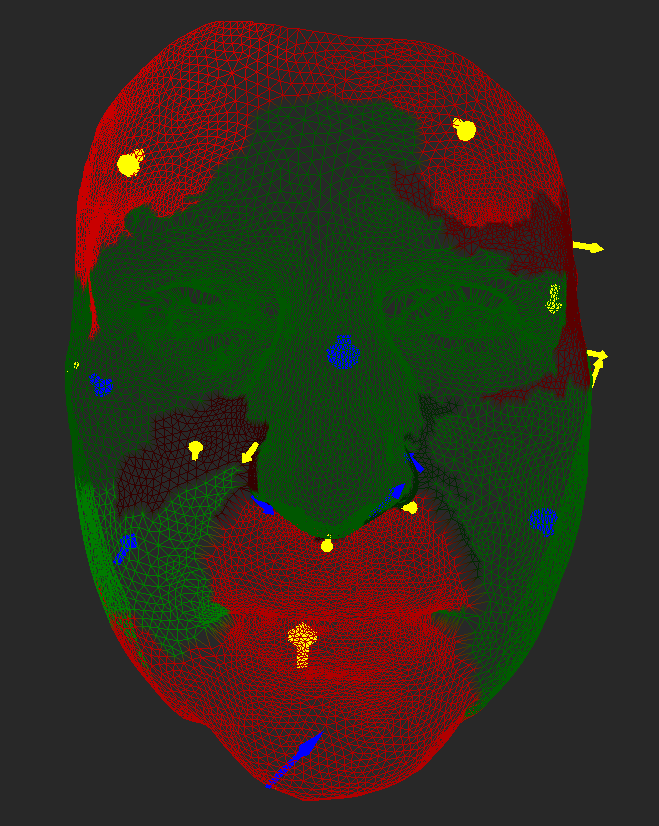
\includegraphics[width=0.5\textwidth]{./img/meshdiff-combination.PNG}
\caption[MeshDiff - Combined visualization]{MeshDiff - Combined visualization}
\label{fig:meshdiff_combination}
\end{figure}

\subsubsection{Expected Performance}

Combined visualizations complement each other in areas when only one visualization is not sufficiently clear. Color visualization is expected to highlight the dimension of the metric we are interested in the most, for example vertex distance magnitude, while arrow visualization is expected to carry other dimensions like direction and cluster size. This method is expected to have a good balance between clarity and information richness.
%%-----------------------------------------------------------------------------------------
%% SECTION
%%-----------------------------------------------------------------------------------------
\section{The Effect of Clustering Parameters}
\label{sec:parameter_effect}

The function used for computing the clustering error (see eq. \ref{eq:clustering_error}) has four parameters:

\begin{itemize}
\item Direction weight
\item Position weight
\item Magnitude weight
\item Resolution weight
\end{itemize}

A specific configuration of these parameters can influence the outcome of the clustering process considerably. In general, setting one of them higher than others results in finer clustering in that dimension and coarser clustering in others. We will now describe the effect of each of the parameters in more detail.

%%-----------------------------------------------------------------------------------------
\subsection{Direction Weight}

High direction weight forms many small clusters in areas of high surface curvature and large clusters in flat areas. Therefore, it mostly captures the high-curvature changes of shape. Resulting clusters have uneven sizes.
%%-----------------------------------------------------------------------------------------
\subsection{Position Weight}

Setting the position weight higher than others results in clusters of even size where each of them represents the overall difference in a certain area regardless of the variety of directions and magnitudes in that area.
%%-----------------------------------------------------------------------------------------
\subsection{Magnitude Weight}

Magnitude weight can play a significant role when using the metric-based cluster color visualization because its high value will highlight iso-magnitude contours like in a geographical map. Such an approach can be useful when grouping and segmenting areas with a certain absolute value of the difference metric.
%%-----------------------------------------------------------------------------------------
\subsection{Resolution Weight}

High resolution weight prefers clustering in sparse areas of the mesh and will therefore increase the precision of the visualization in very dense areas. This effect partially complements high direction weight because high-curvature areas of triangle meshes are usually more dense in order for the high curvature to be captured well in the mesh.

\begin{figure}[h]
\centering
	\begin{subfigure}{0.3\textwidth}
	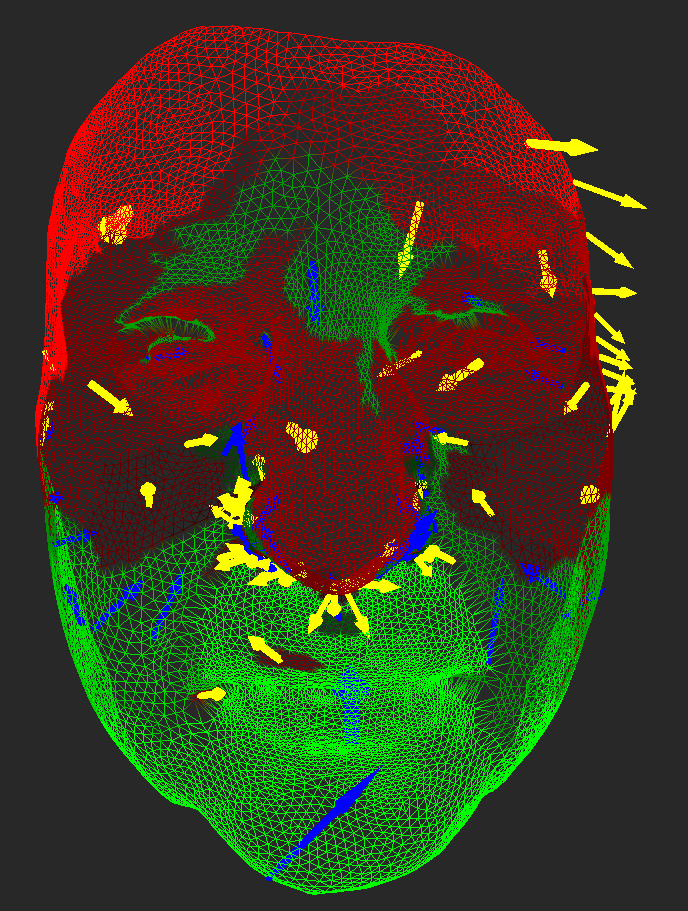
\includegraphics[width=\textwidth]{./img/meshdiff-high_direction.PNG}
	\caption{High direction weight}
	\label{fig:meshdiff_high_direction}
	\end{subfigure}
    \qquad
    \begin{subfigure}{0.3\textwidth}
	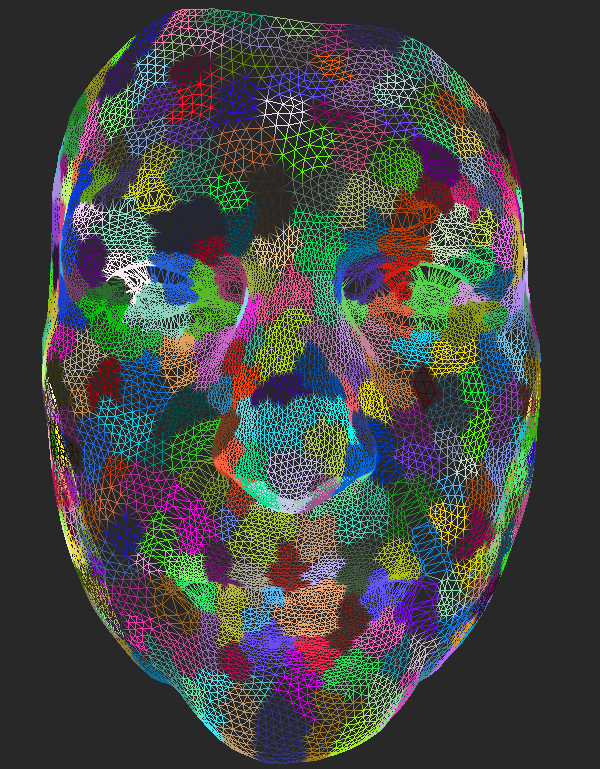
\includegraphics[width=\textwidth]{./img/meshdiff-high_position.PNG}
	\caption{High position weight}
	\label{fig:meshdiff_high_position}
	\end{subfigure}
    
    \begin{subfigure}{0.3\textwidth}
	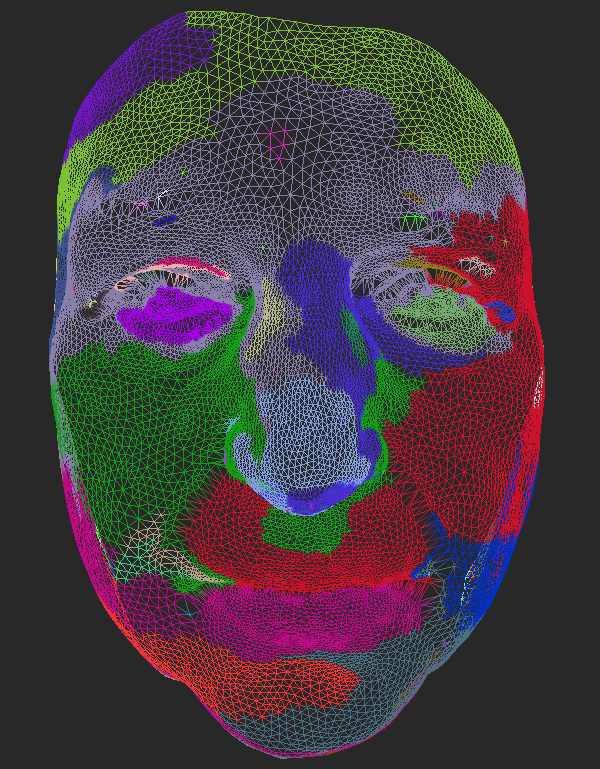
\includegraphics[width=\textwidth]{./img/meshdiff-high_magnitude.PNG}
	\caption{High magnitude weight}
	\label{fig:meshdiff_high_magnitude}
	\end{subfigure}
    \qquad
    \begin{subfigure}{0.3\textwidth}
	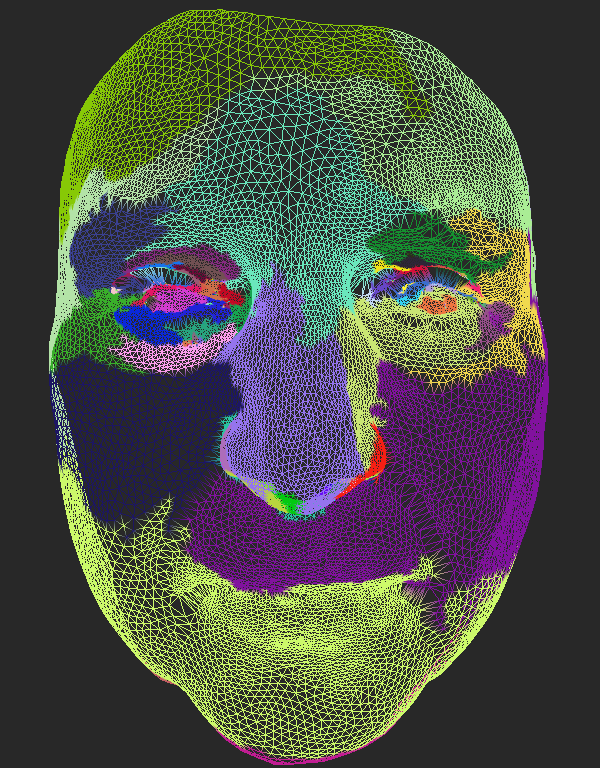
\includegraphics[width=\textwidth]{./img/meshdiff-high_resolution.PNG}
	\caption{High resolution weight}
	\label{fig:meshdiff_high_resolution}
	\end{subfigure}
\caption[MeshDiff - Various clustering parameter settings]{MeshDiff - Various clustering parameter settings}
\end{figure}